\documentclass{standalone}
\usepackage{tikz}
\usepackage{ctex,siunitx}
\setCJKmainfont{Noto Serif CJK SC}
\usepackage{tkz-euclide}
\usepackage{amsmath}
\usetikzlibrary{patterns, calc,3d}
\usetikzlibrary {decorations.pathmorphing,decorations.pathreplacing,decorations.shapes}
\tikzset{label style/.append style={font=\small}}
\begin{document}
\small
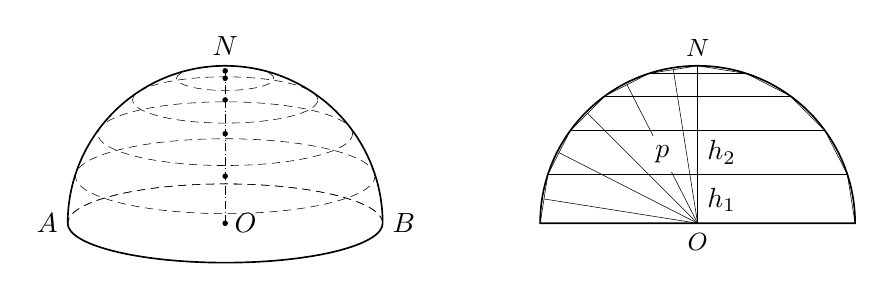
\begin{tikzpicture}[>=latex,scale=1.0]
  \foreach \x in {1,2,3,4}
  {
    \tkzDefPoint(\x*18:2){R\x}
    \tkzDefPoint(180-\x*18:2){L\x}
    \tkzDrawSegments[very thin](R\x,L\x)
  }
  \tkzDefPoints{2/0/R,-2/0/L,0/0/O,0/2/N}
  \draw[very thin](R)--(R1)--(R2)--(R3)--(R4)--(0,2)--(L4)--(L3)--(L2)--(L1)--(L);
  \tkzDefMidPoint(L,L1)\tkzGetPoint{P1}
  \tkzDefMidPoint(L1,L2)\tkzGetPoint{P2}
  \tkzDefMidPoint(L2,L3)\tkzGetPoint{P3}
  \tkzDefMidPoint(L3,L4)\tkzGetPoint{P4}
  \tkzDefMidPoint(L4,N)\tkzGetPoint{P5}
  \draw[semithick](2,0)arc(0:180:2)--cycle;
  \tkzDrawSegments[very thin](O,N O,P1 O,P2 O,P3 O,P4 O,P5)
  \tkzLabelLine[pos=0.15,right](O,N){$h_1$}
  \tkzLabelLine[pos=0.45,right](O,N){$h_2$}
  \tkzLabelLine[pos=0.5,fill=white](O,P4){$p$}
  \tkzLabelPoints(O)
  \tkzLabelPoints[above](N)
\begin{scope}[xshift=-6cm]
  \draw[semithick](2,0)node[right]{$B$}arc(0:180:2)node[left]{$A$};
  \draw[semithick](2,0)arc(0:-180:2 and 0.5);
  \draw[very thin,densely dashed](2,0)arc(0:180:2 and 0.5);
  \foreach \x in {0,1,2,3,4,5}
  {
    \draw[densely dashed,very thin](0,{2*0.968*sin(\x*18)})ellipse( {2*cos(\x*18)} and {0.5*cos(\x*18)});
    \fill(0,{2*0.968*sin(\x*18)})circle(1pt);
  }
  \draw[very thin,densely dashdotted](0,0)node[right]{$O$}--(0,1.936)node[above=2pt]{$N$};
\end{scope}
\end{tikzpicture}
\end{document}